\chapter{Desenho e Prototipagem das Placas Mãe, Placas de Chute e Placas Acionadoras dos Motores dos Robôs}\label{cap:design_placas}

O projeto das placas foi feito em duas etapas. A primeira etapa foi o desenvolvimento do esquemático do circuito, representação simbólica dos componentes e suas ligações. Nessa fase foram selecionados os componentes. A segunda etapa foi o \textit{layout}, em que foi feito um CAD (\textit{Computer Aided Design} ­– desenho assistido por computador) com o posicionamento dos componentes e o desenho das trilhas de cobre, tomando por base o esquemático. Foi preciso levar em conta a corrente que circularia pelo circuito para definir a larguras das trilhas, os tamanhos dos componentes a serem soldados e o tamanho da placa que seria produzida. Ao projetar as placas, os alunos da iniciativa adquirem experiência tanto em desenho de PCBs (\textit{Printed Circuit Board} – placa de circuito impresso), como em soldagem de componentes SMD (\textit{Surface Mounted Device} – dispositivo montado em superfície).

Para o desenvolvimento das placas, foi utilizado o \textit{software} \textit{Altium Designer\textsuperscript{\textregistered}}. As Figuras ~\ref{fig:blocos_placa_mae} apresentam os diagramas de blocos feitos a partir de esboços dos desenhos das três placas, utilizando uma das funcionalidades do \textit{Altium}.

Na placa mãe, o módulo de transmissão envia os dados recebidos da inteligência para o microcontrolador (que fica no módulo de controle adquirido) via protocolo SPI.
O módulo de controle envia sinais PWM para os módulos de motores e um pulso e um sinal digital para o módulo do chute. As correntes nos módulos de motores são medidas por circuitos integrados dedicados e enviadas para o módulo de controle via protocolo I2C.

Para funcionamento dos motores, são usados drivers e uma ponte H, para que os motores possam trabalhar nos dois sentidos.
Feito dessa forma, o \textit{hardware} passa a ter o fluxograma apresentado na Figura\ref{fig:func_hw}. Os comandos chegam através do módulo de comunicação e pela placa mãe é transmitida até a o módulo de controle (\textit{Discovery} STM32F4), que então a envia aos módulos pertinentes, motores ou chute. Há quatro motores ligados às rodas e um ao drible. O chute está separado em forte (baixo) e fraco (alto). Para fazer o controle das velocidades de giro de cada roda, informações sobre as rotações das rodas são passadas para a \textit{Discovery}, que pode também passá-las para o módulo de transmissão, se for o caso.

\begin{figure}
	\centering
	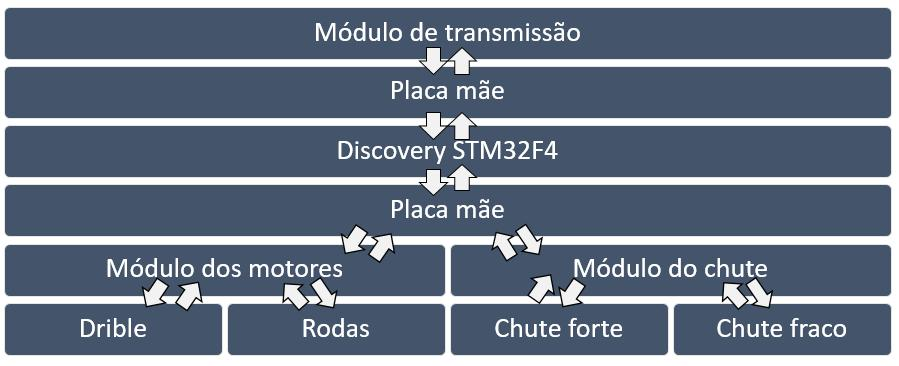
\includegraphics[scale=0.5]{funcionamento_hw}
	\caption{Funcionamento do \textit{hardware}}
	\label{fig:func_hw}
\end{figure}

%\begin{figure}
%	\centering
%	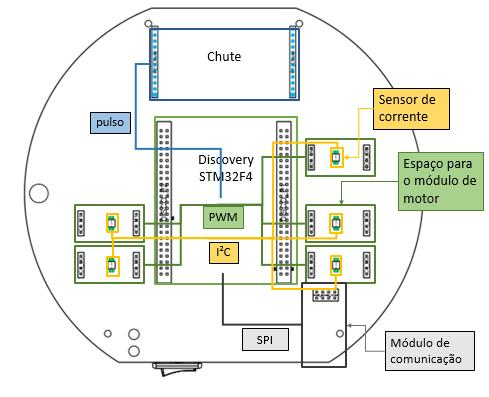
\includegraphics[scale=1]{blocos_placa_mae}
%	\caption{Diagrama de blocos da Placa Mãe}
%	\label{fig:blocos_placa_mae}
%\end{figure}

\section{Placa Mãe}\label{sec:placa_mae}

A placa-mãe (Figura~\ref{fig:modulo_placa_mae}) é responsável por fazer a ligação entre os atuadores do robô, transmitindo potência da bateria para os módulos de motor e de chute, fazendo a ligação entre esses módulos e os respectivos atuadores, fornecendo tensão aos circuitos lógicos e fazendo a ligação entre o módulo de controle e os sensores do robô -, no caso um sensor de quadratura em cada motor e o sensor ótico do chute que verifica a posse da bola. 

\begin{figure}
	\centering
	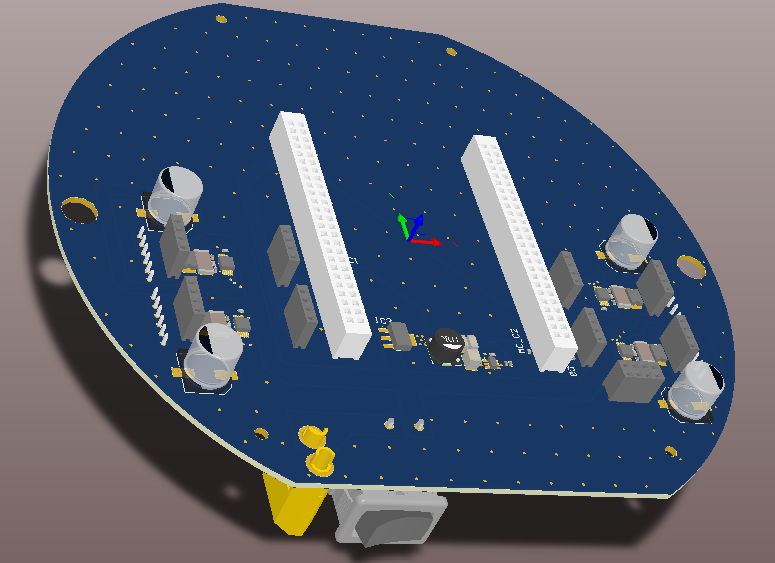
\includegraphics[scale=1]{modulo_placa_mae}
	\caption{Módulo da placa-mãe}
	\label{fig:modulo_placa_mae}
\end{figure}

\begin{figure}
	\centering
	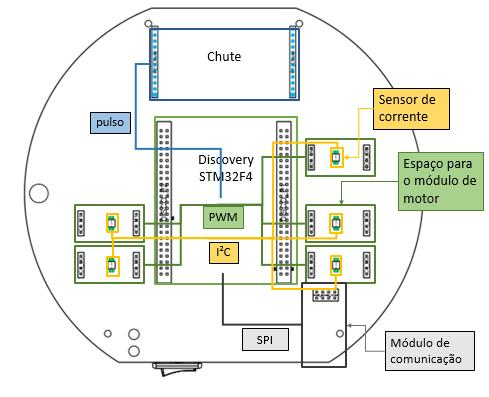
\includegraphics[scale=1]{blocos_placa_mae}
	\caption{Diagrama de blocos da placa mãe}
	\label{fig:blocos_placa_mae}
\end{figure}

Para que as conexões elétricas através da placa sejam feitas de modo seguro, a placa mãe contém um fusível, um capacitor de tanque, um capacitor de desacoplamento, e um sensor de corrente, o chip INA220, na entrada de cada módulo de motor e na entrada do módulo de chute, além de um circuito de divisão de tensão para que o módulo de controle seja capaz de controlar o nível de tensão da bateria.
O controle dessa placa é feito no firmware através da classe INA220, que faz a comunicação com os sensores de corrente na placa e a classe bateria que controla o nível da bateria sendo usada pelo robô. Essas classes permitem o controle dos circuitos de segurança do robô de maneira que o firmware possa lidar com comportamentos anômalos.
O desenho dessa placa foi reformulado:

\begin{itemize}
  \item As trilhas nos caminhos de potência foram trocados por planos para diminuir a resistência e o aquecimento das trilhas;
  \item Os antigos fusíveis simples foram trocados por fusíveis resetáveis para evitar que precisasse ser trocado durante a competição ou a 		cada sobrecorrente;
  \item Os antigos capacitores de tanque through hole foram trocados por capacitores SMD visando automatizar o processo de montagem utilizando 			uma pick and place automática;
  \item Os sensores de corrente também foram trocados por sua versão mais moderna e foi corrigido um erro no esquemático da placa mãe;
  \item O conector do módulo de transmissão foi trocado para ser compatível com o novo módulo de transmissão adotado pelo time.
\end{itemize}

% vim: tw=80 et ts=2 sw=2 sts=2 ft=tex spelllang=pt_br,en

\section{Módulo do Motor}\label{sec:modulo_motor}

Os módulos de motor (Figura~\ref{fig:modulo_motor}) fazem o controle dos quatro motores responsáveis pelo movimento do robô e do motor responsável pela atuação do driblador. Cada módulo consiste em uma ponte H capaz de controlar a velocidade de um motor de corrente contínua em duas direções. 

\begin{figure}
	\centering
	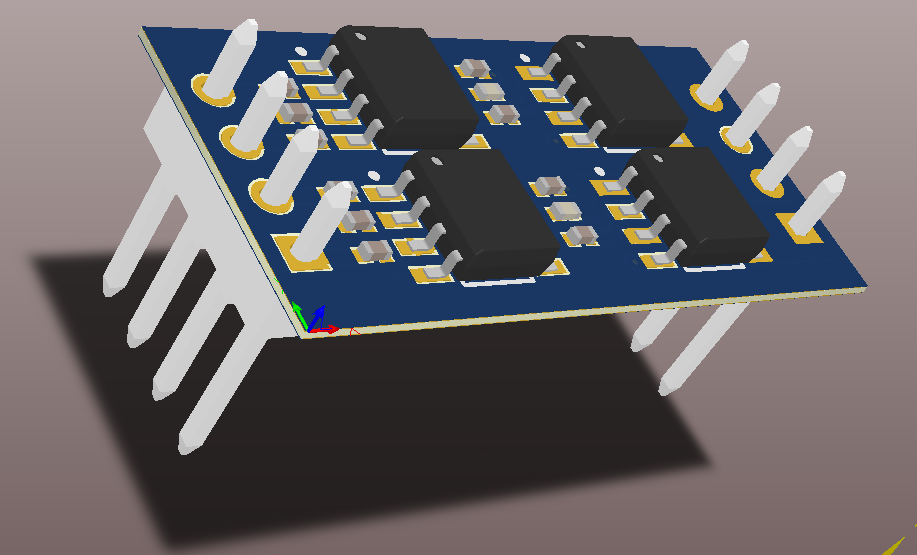
\includegraphics[scale=1]{modulo_motor}
	\caption{Módulo de Motor}
	\label{fig:modulo_motor}
\end{figure}

\begin{figure}
	\centering
	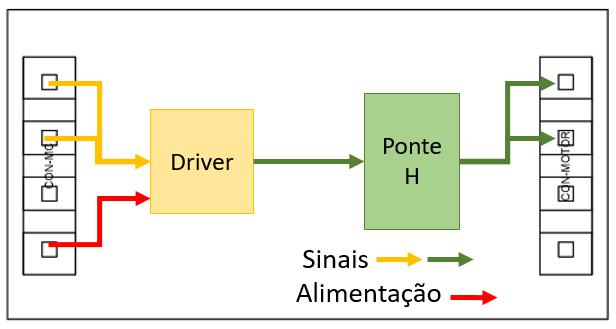
\includegraphics[scale=1]{blocos_motor}
	\caption{Diagrama de blocos do módulo de motor}
	\label{fig:blocos_motor}
\end{figure}

Esta placa é controlada pelo módulo de controle através da classe motor que utiliza a classe encoder para determinar a velocidade instantânea do motor. Com essa velocidade utiliza-se um algoritmo de controle PID para calcular a resposta que deve ser transmitida à placa, e envia-se essa resposta utilizando as classes degrau unitário e PWM.
O circuito de ponte H permite que o microcontrolador controle o sentido de rotação dos motores e a potência transmitida a eles, através do chaveamento dos transistores internos da ponte e amplificando o sinal enviado pelo microcontrolador.
O desenho dessa placa foi reformulado esse ano, as trilhas foram trocadas por planos nos caminhos de potência e foram adicionados um par de capacitores de desacoplamento na entrada dos drivers dos transistores.


% vim: tw=80 et ts=2 sw=2 sts=2 ft=tex spelllang=pt_br,en

\section{Módulo do Chute}\label{sec:modulo_chute}

O mecanismo de chute do robô foi elaborado utilizando dois solenóides como atuadores, um responsável pelo chute para frente e outro responsável pelo chute alto. E a placa (Figura~\ref{fig:modulo_chute}) é responsável por produzir a alta tensão necessária para ativar os dois solenóides, e transmitir a energia acumulada para acionar os atuadores.

\begin{figure}
	\centering
	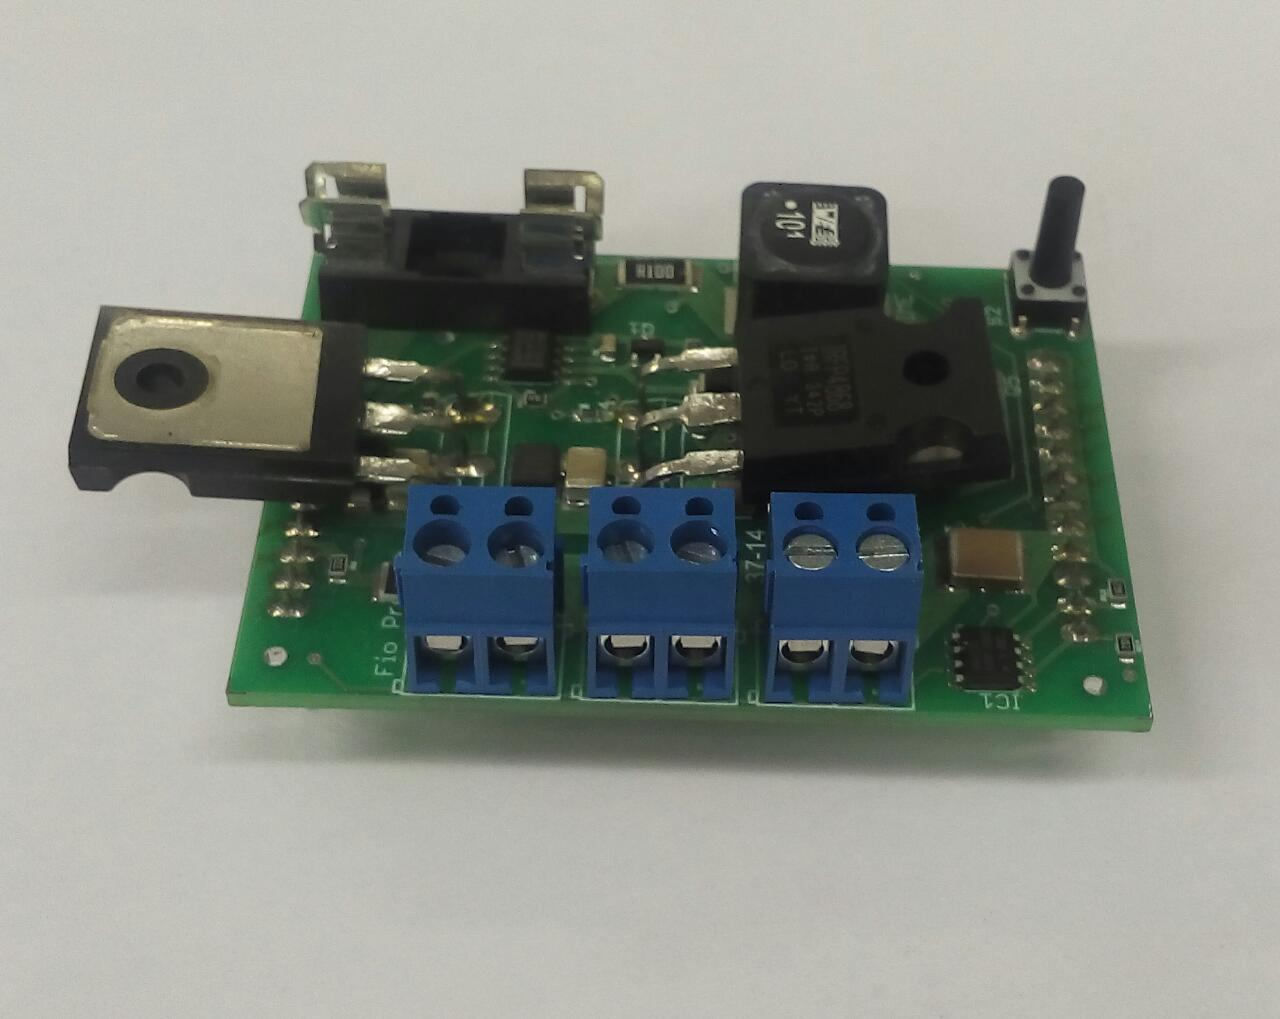
\includegraphics[scale=1]{modulo_chute}
	\caption{Módulo do Chute}
	\label{fig:modulo_chute}
\end{figure}

A placa funciona através de um circuito de conversão DC-DC controlado pelo circuito integrado MC34063 que converte os 7,8V DC da bateria em uma saída de 180V DC ligada a dois capacitores eletrolíticos de 2200 $\mu$F e 200V. Além desse circuito existe ainda um circuito para chavear a tensão dos capacitores nos solenóides, o que é feito utilizando um TC4427 driver de MOSFET e dois MOSFETs de potência IRFP4868PBF. 
O controle desse módulo é feito através da classe chute que utiliza a classe degrau unitário para limitar a energia transmitida a bola alterando a duração do intervalo de tempo que os MOSFETs ficarão ativados.

\begin{figure}
	\centering
	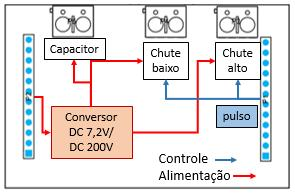
\includegraphics[scale=1]{blocos_chute}
	\caption{Diagrama de blocos do módulo de chute}
	\label{fig:blocos_chute}
\end{figure}


% vim: tw=80 et ts=2 sw=2 sts=2 ft=tex spelllang=pt_br,en


% Ramificação constante ou taxa constante

% vim: tw=80 et ts=2 sw=2 sts=2 ft=tex spelllang=pt_br,en
